\documentclass[11pt]{article}
\usepackage[margin=1in]{geometry}
\usepackage{amsmath,amssymb}
\usepackage{graphicx}
\usepackage{booktabs}
\usepackage{float}
\usepackage{caption}
\usepackage{hyperref}
\usepackage{xcolor}
\graphicspath{{figures/}}
\captionsetup{font=small,labelfont=bf}
\hypersetup{colorlinks,linkcolor=blue!60!black,citecolor=blue!60!black,urlcolor=blue!60!black}

\newcommand{\Real}{\operatorname{Re}}
\newcommand{\Imag}{\operatorname{Im}}
\newcommand{\infbeyn}{InfBeyn}

\title{Spectral stability of non-transonic plasma flows in the magnetic nozzle,\\
revisited with the infinite-dimensional Beyn method}
\author{Hunt Feng}
\date{\today}

\begin{document}
\maketitle

\begin{abstract}
The polynomial eigenvalue problem of the thesis \cite{feng2024} for plasma flow in a magnetic nozzle is
solved again for the four non-transonic configurations (constant and spatially varying velocity, subsonic
and supersonic, each with Dirichlet and fixed-open boundary conditions) using \infbeyn{}, the contour-integral
method of Colbrook and Townsend \cite{colbrook2023} applied directly to the differential operator. The
method returns every eigenvalue in a prescribed window of the complex plane, and each one is certified
through the pseudospectral quantity $\gamma_n$. There are no spurious eigenvalues and no convergence test
is required. The stability verdicts of the thesis are confirmed: both subsonic and supersonic flows are
stable with Dirichlet boundaries, the supersonic flow is unstable with fixed-open boundaries, and the
subsonic flow with a varying velocity profile has a single unstable ground mode with fixed-open boundaries.
The new eigenvalues are compared with the thesis-era finite-difference, spectral-collocation and
spectral-Galerkin results. For the constant-velocity problems \infbeyn{} agrees with the exact eigenvalues to
$10^{-13}$. Finite differences on $N=101$ and $N=201$ points miss the eigenvalues by $10^{-3}$ to $10^{0}$
and produce up to eight spurious eigenvalues in the window; collocation agrees with \infbeyn{} to
$10^{-13}$ for constant velocity, to $10^{-11}$ for the varying profiles with Dirichlet boundaries and to
$10^{-3}$ with fixed-open boundaries.
\end{abstract}

\section{Problem}

The linearized flow equations of the thesis reduce to the quadratic eigenvalue problem (thesis Eq.~3.6)
\begin{equation}
  T(\omega)\tilde v \equiv
  \omega^2 \tilde v + 2i\omega\left(v_0\tilde v' + v_0'\tilde v\right)
  + \left[(1-v_0^2)\tilde v'' - \Big(3v_0+\frac1{v_0}\Big)v_0'\tilde v'
  - \Big(1-\frac1{v_0^2}\Big)v_0'^2\tilde v - \Big(v_0+\frac1{v_0}\Big)v_0''\tilde v\right] = 0
  \label{eq:nep}
\end{equation}
on $z\in[-1,1]$, with either Dirichlet boundaries $\tilde v(-1)=\tilde v(1)=0$ or fixed-open boundaries
$\tilde v(-1)=\tilde v'(1)=0$. A mode grows in time when $\Imag\omega>0$.
The equilibrium velocity is (thesis Eq.~2.33)
\begin{equation}
  v_0(z) = \left[-W_k\!\left(-\frac{B(z)^2}{B_m^2}v_m^2 e^{-v_m^2}\right)\right]^{1/2},\qquad
  B(z) = B_0\left(1+R\,e^{-(z/\Delta)^2}\right),
\end{equation}
with $B_0=1$, $R=1.5$, $\Delta=1/3$, $B_m=B(0)$, and the Lambert branch $k=0$ for the subsonic profile
($v_m=0.5$) and $k=-1$ for the supersonic profile ($v_m=1.5$). The derivatives $v_0'$, $v_0''$ are evaluated
exactly from the equilibrium relation $(v_0^2-1)v_0' = -v_0B'/B$. The constant-velocity cases use
$v_0\equiv v_m$. Figure~\ref{fig:v0} shows the four profiles.

\begin{figure}[H]
  \centering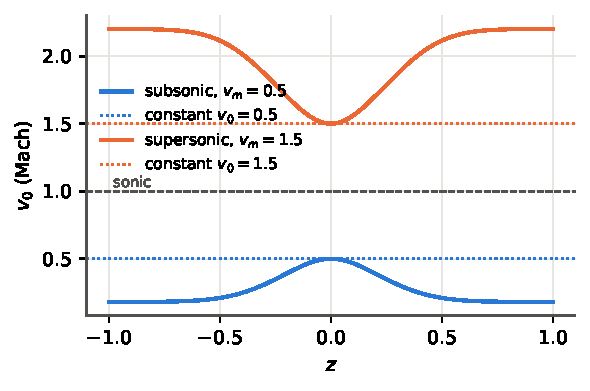
\includegraphics[width=0.6\textwidth]{velocity_profiles}
  \caption{Equilibrium velocity profiles of the eight cases: constant ($v_0=0.5$, $1.5$) and spatially
  varying ($v_m=0.5$, $1.5$ at the throat $z=0$).}
  \label{fig:v0}
\end{figure}

For constant velocity the eigenvalues are known in closed form (thesis Eqs.~3.10 and 3.12):
\begin{align}
  \text{Dirichlet:}\quad &\omega_n = \frac{n\pi}{2}(1-v_0^2),\qquad n=\pm1,\pm2,\dots \label{eq:exactD}\\
  \text{fixed-open:}\quad &\omega_n = (v_0^2-1)\left[\phi_n - \frac{i}{4}\ln\left|\frac{v_0-1}{v_0+1}\right|\right],
  \qquad \phi_n = \begin{cases} n\pi/2, & v_0>1,\\ (2n+1)\pi/4, & v_0<1.\end{cases} \label{eq:exactFO}
\end{align}
Two remarks on Eq.~\eqref{eq:exactFO}. The condition $\tilde v'(1)=0$ gives
$e^{-4i\omega/(v_0^2-1)} = (1+v_0)/(v_0-1)$; for $v_0<1$ the right-hand side is negative, so its logarithm
carries an extra $i\pi$ and the real parts sit at half-integer multiples of $\pi(1-v_0^2)/2$. Thesis
Eq.~(3.12) writes $n\pi/2$ for both signs, but the values plotted in thesis Fig.~3.2(a)
($\Real\omega = -0.589, -1.767, \dots$) already correspond to the half-integer phases $\phi_n$ used here. Secondly,
$n=0$ in Eq.~\eqref{eq:exactD} gives $\omega=0$ with $\tilde v\equiv0$ (thesis Eq.~3.9), so it is not an
eigenvalue and is excluded.

\section{Method}

\infbeyn{} \cite{colbrook2023} is Beyn's contour method applied to the operator $T(\omega)$ itself. For a closed
contour $\Gamma$ one forms the quasimatrices
\begin{equation}
  A_0 = \frac1{2\pi i}\oint_\Gamma T(z)^{-1}V\,dz,\qquad
  A_1 = \frac1{2\pi i}\oint_\Gamma z\,T(z)^{-1}V\,dz,
\end{equation}
where $V$ is a set of random smooth test functions. Each $T(z)^{-1}V$ is a linear boundary value problem,
solved by Chebyshev collocation with the number of points doubled until the Chebyshev coefficients of the
solution have decayed below $10^{-12}$. The eigenvalues inside $\Gamma$ are those of the small matrix pencil
obtained from the SVD of $A_0$. Only linear BVPs are ever discretized, each to its own tolerance, so there is
no global discretization of the eigenvalue problem and hence no spectral pollution.

The implementation (\texttt{inf\_beyn.py}) was used as follows for every case:
\begin{itemize}
  \item \texttt{scan()} over the window $\Real\omega\in[-0.5,26]$, $\Imag\omega\in[-3,3]$ by adaptive
  rectangular subdivision (Clenshaw--Curtis rule with 33 nodes per edge, up to 7 levels, 24 test functions).
  A tile is accepted only if the singular values of $A_0$ show a gap of at least $10^4$ and the nested
  half rule reproduces the eigenvalues. Accepted estimates are polished by Newton's method on the bordered
  system $[T(\omega)u;\,c^*u-1]=0$ on a grid doubled until convergence.
  \item \texttt{verify()}: for each eigenvalue, $\gamma_n(\omega)=\min_u\|T(\omega)u\|/\|u\|$ over
  polynomials of degree $n=64,128,256$ satisfying the boundary conditions. By Theorem~2.2 of
  \cite{colbrook2023} $\omega$ lies in the $\gamma_n(\omega)$-pseudospectrum of $T$; a true, well-conditioned
  eigenvalue has $\gamma_n(\omega)$ at rounding level and a much larger ``halo'' value of $\gamma_n$ on a
  circle (radius $0.25$) around it.
  \item \texttt{pseudospectra()}: $\gamma_{128}$ on a $265\times61$ grid of the window.
\end{itemize}
The old technique of the thesis is also rerun on the same operator: second-order central finite differences
on $N=101$ and $N=201$ equispaced points, with $\tilde v'(1)=0$ imposed by a one-sided second-order stencil,
linearized to a generalized eigenvalue problem (\texttt{nozzle\_infbeyn.py}, function
\texttt{finite\_difference}). The spectral-collocation ($N=101$ Chebyshev points) and spectral-Galerkin
(30 compact Legendre combinations) eigenvalues are taken unchanged from the thesis data files in
\texttt{../data/}. These three contain all eigenvalues of the discretized problem, spurious ones included;
the thesis removed the spurious ones by a convergence test. Here an old eigenvalue in the window farther than
$0.1$ from every \infbeyn{} eigenvalue is counted as spurious.

Running all eight cases takes about two and a half minutes on 12 cores (forked workers); the scans
themselves take 2 to 9 seconds each (Table~\ref{tab:summary}).

\section{Results}

\begin{table}[H]
  \centering\small
  \begin{tabular}{llrrrll}
\toprule
case & BC & \#eig & BVP solves & scan [s] & $\max\,\mathrm{Im}\,\omega$ (mode) & verdict\\
\midrule
constant $v_0=0.5$ & Dirichlet & 22 & 5062 & 3 & $0.0000$ ($8.247+0.000i$) & stable\\
constant $v_0=0.5$ & fixed-open & 22 & 1858 & 2 & $-0.2060$ ($18.261-0.206i$) & stable\\
constant $v_0=1.5$ & Dirichlet & 13 & 1167 & 2 & $0.0000$ ($25.525+0.000i$) & stable\\
constant $v_0=1.5$ & fixed-open & 14 & 790 & 2 & $0.5029$ ($-0.000+0.503i$) & unstable\\
$v_m=0.5$ & Dirichlet & 18 & 3617 & 8 & $0.0000$ ($5.718+0.000i$) & stable\\
$v_m=0.5$ & fixed-open & 18 & 3680 & 9 & $0.0388$ ($0.647+0.039i$) & unstable\\
$v_m=1.5$ & Dirichlet & 6 & 413 & 3 & $0.0000$ ($24.683+0.000i$) & stable\\
$v_m=1.5$ & fixed-open & 7 & 413 & 8 & $1.0136$ ($0.000+1.014i$) & unstable\\
\bottomrule
\end{tabular}

  \caption{Summary of the \infbeyn{} scans. Eigenvalue counts are for the window $\Real\omega\in[-0.5,26]$,
  $\Imag\omega\in[-3,3]$; the growth rate is the largest $\Imag\omega$ found and the mode that attains it.}
  \label{tab:summary}
\end{table}

Every eigenvalue of every case passed the certification: $\gamma_{256}(\omega)\le 3\times10^{-8}$ (at
the rounding floor of the computation) with a halo larger by seven to ten orders of magnitude, and the
pseudospectral plots show no region of small $\gamma_n$ other than the isolated discs around the eigenvalues.
No tile was left unresolved. The stability verdicts of the thesis are reproduced in all eight cases.

\subsection{Constant velocity}

\paragraph{Subsonic, $v_0=0.5$.} With Dirichlet boundaries the 22 eigenvalues in the window are real
and equal to $n\pi(1-v_0^2)/2$ to within $10^{-13}$ (Fig.~\ref{fig:css}, Table~\ref{tab:css}). With fixed-open
boundaries all 22 eigenvalues share the damping rate $\Imag\omega = -0.2060 = \frac{3}{16}\ln\frac13$
(Fig.~\ref{fig:cso}, Table~\ref{tab:cso}); the flow is stable.

\paragraph{Supersonic, $v_0=1.5$.} Dirichlet: 13 real eigenvalues $n\pi(v_0^2-1)/2$, stable
(Fig.~\ref{fig:cSs}, Table~\ref{tab:cSs}). Fixed-open: 14 eigenvalues with the common growth rate
$\Imag\omega = 0.50295 = \frac{5}{16}\ln 5$, including the purely imaginary $n=0$ mode; the flow is unstable
(Fig.~\ref{fig:cSo}, Table~\ref{tab:cSo}). The $n=0$ eigenvalue is matched to $2\times10^{-11}$, the others
to $10^{-12}$; its eigenfunction is the smoothest but the resolvent is largest there.

\begin{figure}[H]
  \centering
  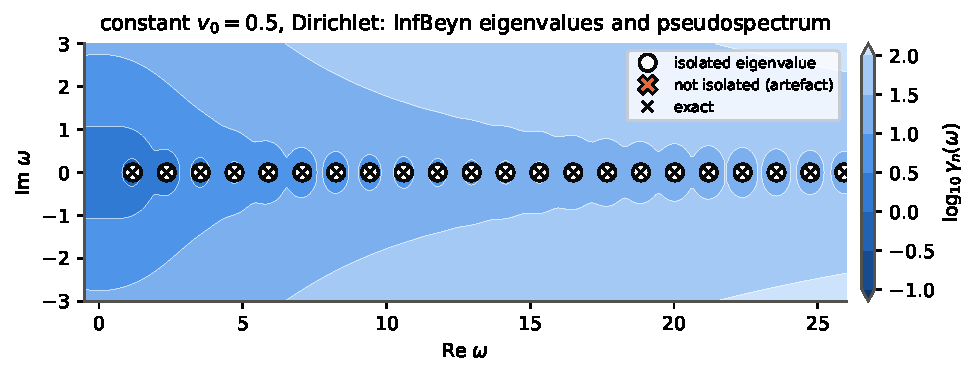
\includegraphics[width=\textwidth]{constant_subsonic_fixed_fixed_spectrum}\\
  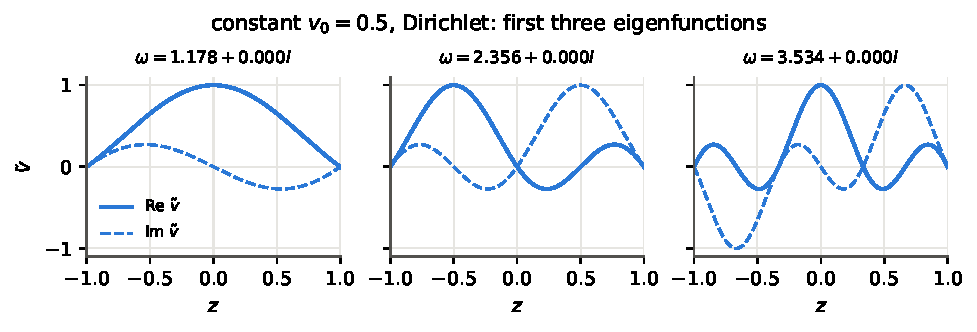
\includegraphics[width=\textwidth]{constant_subsonic_fixed_fixed_eigenfunctions}
  \caption{Constant $v_0=0.5$, Dirichlet. Top: \infbeyn{} eigenvalues (circles) on the pseudospectrum
  $\log_{10}\gamma_{128}(\omega)$; crosses are the exact eigenvalues. Bottom: first three eigenfunctions
  (Chebyshev series returned by the method, normalized so the largest value is 1).}
  \label{fig:css}
\end{figure}
\begin{table}[H]\centering\footnotesize\begin{tabular}{rlllll}
\toprule
$n$ & $\omega_n$ (InfBeyn) & $\gamma_{256}(\omega_n)$ & halo & polished & $|\omega_n-\omega_n^{\rm exact}|$\\
\midrule
1 & $1.17809725+0.00000000i$ & $6.5\times10^{-10}$ & $7.0\times10^{-1}$ & yes & $2.9\times10^{-14}$\\
2 & $2.35619449+0.00000000i$ & $6.5\times10^{-10}$ & $1.5\times10^{0}$ & yes & $3.5\times10^{-14}$\\
3 & $3.53429174+0.00000000i$ & $6.2\times10^{-10}$ & $2.3\times10^{0}$ & yes & $7.8\times10^{-14}$\\
4 & $4.71238898-0.00000000i$ & $7.0\times10^{-10}$ & $3.1\times10^{0}$ & yes & $2.4\times10^{-14}$\\
5 & $5.89048623-0.00000000i$ & $6.4\times10^{-10}$ & $3.8\times10^{0}$ & yes & $3.6\times10^{-14}$\\
6 & $7.06858347-0.00000000i$ & $6.8\times10^{-10}$ & $4.6\times10^{0}$ & yes & $4.1\times10^{-14}$\\
7 & $8.24668072+0.00000000i$ & $6.9\times10^{-10}$ & $5.4\times10^{0}$ & yes & $2.0\times10^{-14}$\\
8 & $9.42477796-0.00000000i$ & $6.5\times10^{-10}$ & $6.2\times10^{0}$ & yes & $2.0\times10^{-14}$\\
9 & $10.60287521-0.00000000i$ & $6.1\times10^{-10}$ & $6.9\times10^{0}$ & yes & $1.4\times10^{-14}$\\
10 & $11.78097245-0.00000000i$ & $6.9\times10^{-10}$ & $7.7\times10^{0}$ & yes & $3.1\times10^{-14}$\\
\bottomrule
\end{tabular}

  \caption{Constant $v_0=0.5$, Dirichlet: first ten eigenvalues, certification and error.}\label{tab:css}\end{table}

\begin{figure}[H]
  \centering
  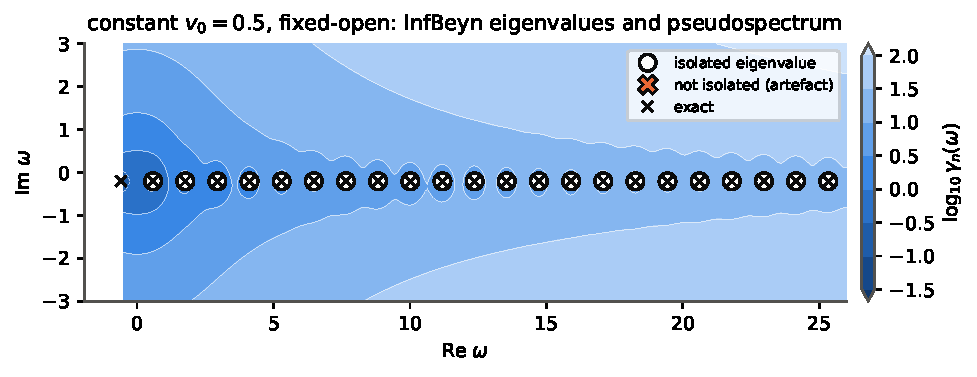
\includegraphics[width=\textwidth]{constant_subsonic_fixed_open_spectrum}\\
  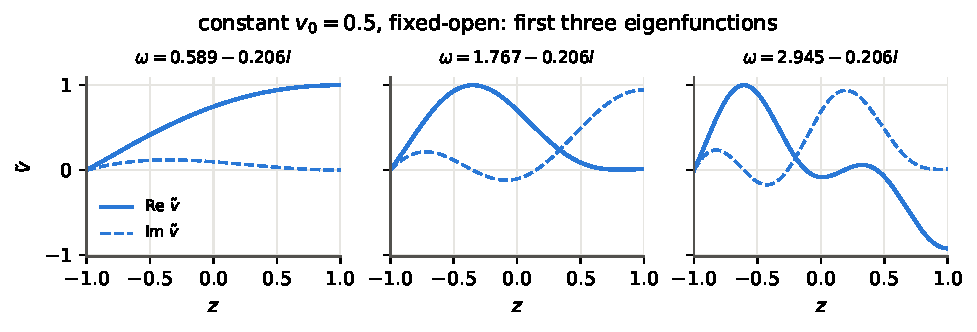
\includegraphics[width=\textwidth]{constant_subsonic_fixed_open_eigenfunctions}
  \caption{Constant $v_0=0.5$, fixed-open.}
  \label{fig:cso}
\end{figure}
\begin{table}[H]\centering\footnotesize\begin{tabular}{rlllll}
\toprule
$n$ & $\omega_n$ (InfBeyn) & $\gamma_{256}(\omega_n)$ & halo & polished & $|\omega_n-\omega_n^{\rm exact}|$\\
\midrule
1 & $0.58904862-0.20598980i$ & $9.0\times10^{-10}$ & $2.7\times10^{-1}$ & yes & $4.1\times10^{-12}$\\
2 & $1.76714587-0.20598980i$ & $7.0\times10^{-10}$ & $8.3\times10^{-1}$ & yes & $1.8\times10^{-12}$\\
3 & $2.94524311-0.20598980i$ & $9.1\times10^{-10}$ & $1.4\times10^{0}$ & yes & $9.6\times10^{-13}$\\
4 & $4.12334036-0.20598980i$ & $8.4\times10^{-10}$ & $2.0\times10^{0}$ & yes & $2.4\times10^{-14}$\\
5 & $5.30143760-0.20598980i$ & $7.0\times10^{-10}$ & $2.6\times10^{0}$ & yes & $9.0\times10^{-13}$\\
6 & $6.47953485-0.20598980i$ & $7.4\times10^{-10}$ & $3.2\times10^{0}$ & yes & $3.0\times10^{-14}$\\
7 & $7.65763209-0.20598980i$ & $7.5\times10^{-10}$ & $3.8\times10^{0}$ & yes & $5.9\times10^{-13}$\\
8 & $8.83572934-0.20598980i$ & $7.6\times10^{-10}$ & $4.4\times10^{0}$ & yes & $1.7\times10^{-13}$\\
9 & $10.01382658-0.20598980i$ & $8.5\times10^{-10}$ & $5.0\times10^{0}$ & yes & $3.2\times10^{-13}$\\
10 & $11.19192383-0.20598980i$ & $7.9\times10^{-10}$ & $5.6\times10^{0}$ & yes & $4.0\times10^{-13}$\\
\bottomrule
\end{tabular}

  \caption{Constant $v_0=0.5$, fixed-open: first ten eigenvalues. The exact values are Eq.~\eqref{eq:exactFO}
  with the half-integer phases.}\label{tab:cso}\end{table}

\begin{figure}[H]
  \centering
  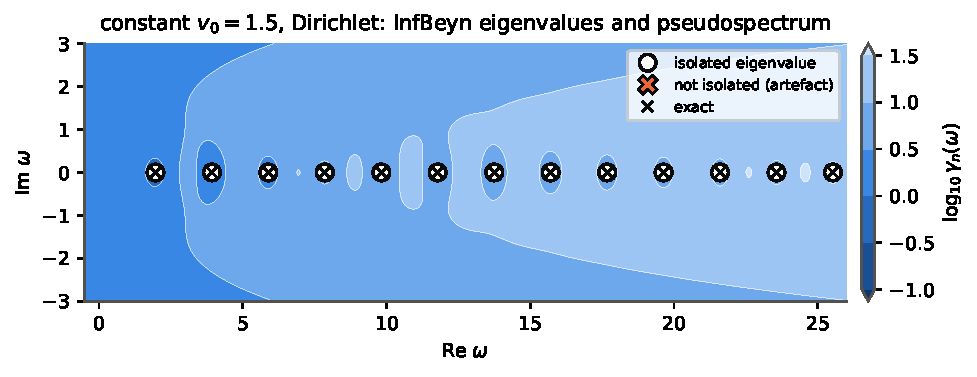
\includegraphics[width=\textwidth]{constant_supersonic_fixed_fixed_spectrum}\\
  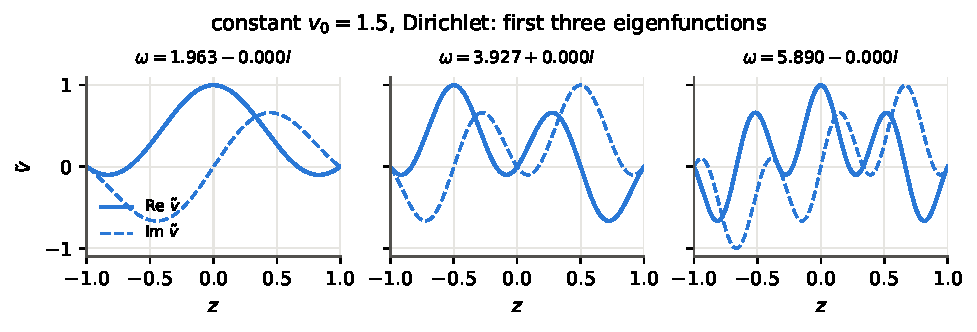
\includegraphics[width=\textwidth]{constant_supersonic_fixed_fixed_eigenfunctions}
  \caption{Constant $v_0=1.5$, Dirichlet.}
  \label{fig:cSs}
\end{figure}
\begin{table}[H]\centering\footnotesize\begin{tabular}{rlllll}
\toprule
$n$ & $\omega_n$ (InfBeyn) & $\gamma_{256}(\omega_n)$ & halo & polished & $|\omega_n-\omega_n^{\rm exact}|$\\
\midrule
1 & $1.96349541-0.00000000i$ & $2.1\times10^{-9}$ & $7.4\times10^{-1}$ & yes & $3.0\times10^{-13}$\\
2 & $3.92699082+0.00000000i$ & $1.9\times10^{-9}$ & $1.5\times10^{0}$ & yes & $5.8\times10^{-14}$\\
3 & $5.89048623-0.00000000i$ & $2.2\times10^{-9}$ & $2.2\times10^{0}$ & yes & $1.1\times10^{-13}$\\
4 & $7.85398163-0.00000000i$ & $2.1\times10^{-9}$ & $3.0\times10^{0}$ & yes & $2.8\times10^{-14}$\\
5 & $9.81747704+0.00000000i$ & $2.0\times10^{-9}$ & $3.7\times10^{0}$ & yes & $7.1\times10^{-14}$\\
6 & $11.78097245-0.00000000i$ & $1.8\times10^{-9}$ & $4.4\times10^{0}$ & yes & $3.5\times10^{-14}$\\
7 & $13.74446786-0.00000000i$ & $2.0\times10^{-9}$ & $5.2\times10^{0}$ & yes & $7.6\times10^{-14}$\\
8 & $15.70796327-0.00000000i$ & $1.8\times10^{-9}$ & $5.9\times10^{0}$ & yes & $5.2\times10^{-14}$\\
9 & $17.67145868-0.00000000i$ & $2.2\times10^{-9}$ & $6.7\times10^{0}$ & yes & $3.0\times10^{-13}$\\
10 & $19.63495408+0.00000000i$ & $2.1\times10^{-9}$ & $7.4\times10^{0}$ & yes & $2.3\times10^{-13}$\\
\bottomrule
\end{tabular}

  \caption{Constant $v_0=1.5$, Dirichlet: first ten eigenvalues.}\label{tab:cSs}\end{table}

\begin{figure}[H]
  \centering
  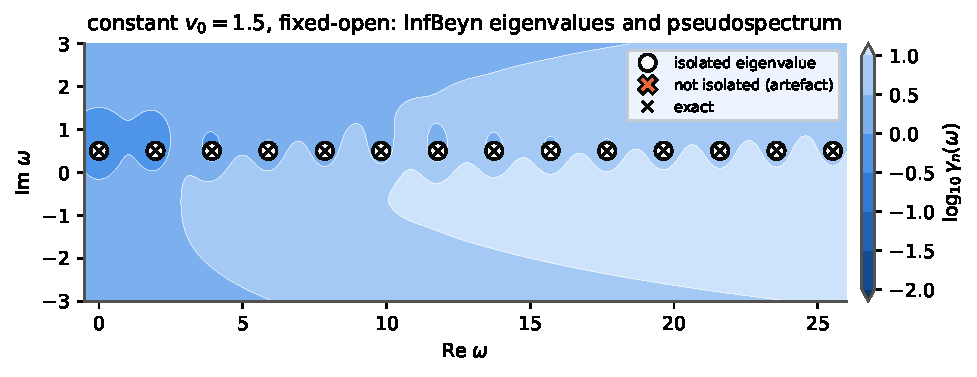
\includegraphics[width=\textwidth]{constant_supersonic_fixed_open_spectrum}\\
  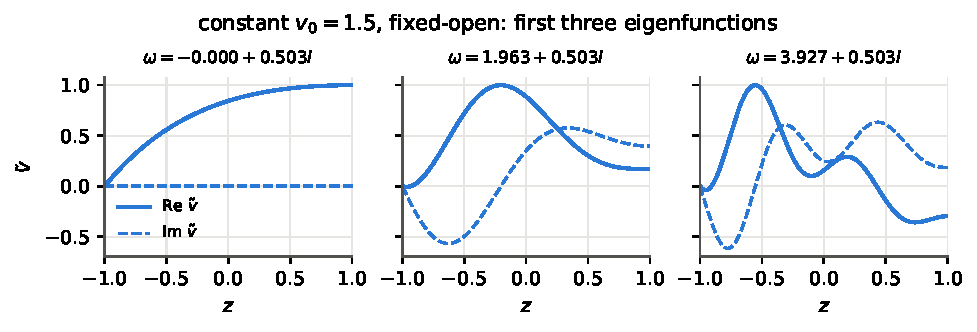
\includegraphics[width=\textwidth]{constant_supersonic_fixed_open_eigenfunctions}
  \caption{Constant $v_0=1.5$, fixed-open. All modes grow at the same rate $\Imag\omega=0.503$.}
  \label{fig:cSo}
\end{figure}
\begin{table}[H]\centering\footnotesize\begin{tabular}{rlllll}
\toprule
$n$ & $\omega_n$ (InfBeyn) & $\gamma_{256}(\omega_n)$ & halo & polished & $|\omega_n-\omega_n^{\rm exact}|$\\
\midrule
1 & $-0.00000000+0.50294935i$ & $1.0\times10^{-9}$ & $3.4\times10^{-1}$ & yes & $2.1\times10^{-11}$\\
2 & $1.96349541+0.50294935i$ & $7.5\times10^{-10}$ & $4.0\times10^{-1}$ & yes & $1.7\times10^{-12}$\\
3 & $3.92699082+0.50294935i$ & $6.1\times10^{-10}$ & $6.8\times10^{-1}$ & yes & $1.2\times10^{-12}$\\
4 & $5.89048623+0.50294935i$ & $7.3\times10^{-10}$ & $9.9\times10^{-1}$ & yes & $9.3\times10^{-13}$\\
5 & $7.85398163+0.50294935i$ & $9.2\times10^{-10}$ & $1.3\times10^{0}$ & yes & $9.5\times10^{-14}$\\
6 & $9.81747704+0.50294935i$ & $8.9\times10^{-10}$ & $1.6\times10^{0}$ & yes & $3.0\times10^{-13}$\\
7 & $11.78097245+0.50294935i$ & $8.1\times10^{-10}$ & $1.9\times10^{0}$ & yes & $1.6\times10^{-13}$\\
8 & $13.74446786+0.50294935i$ & $7.9\times10^{-10}$ & $2.2\times10^{0}$ & yes & $1.0\times10^{-12}$\\
9 & $15.70796327+0.50294935i$ & $6.8\times10^{-10}$ & $2.6\times10^{0}$ & yes & $8.7\times10^{-13}$\\
10 & $17.67145868+0.50294935i$ & $7.9\times10^{-10}$ & $2.9\times10^{0}$ & yes & $8.3\times10^{-13}$\\
\bottomrule
\end{tabular}

  \caption{Constant $v_0=1.5$, fixed-open: first ten eigenvalues.}\label{tab:cSo}\end{table}

\subsection{Spatially varying velocity}

\paragraph{Subsonic, $v_m=0.5$.} Dirichlet: 18 real eigenvalues, the first being $\omega_1=1.0562$;
the flow is stable (Fig.~\ref{fig:ss}, Table~\ref{tab:ss}). Fixed-open: the ground mode
$\omega_1 = 0.64662 + 0.03884i$ is unstable, the second mode is strongly damped
($\Imag\omega_2=-0.2709$), and all higher modes are damped with $\Imag\omega\to-0.0825$
(Fig.~\ref{fig:so}, Table~\ref{tab:so}). This is exactly the ``stable except the ground mode'' picture of
thesis Fig.~4.17; the growth rate of the ground mode is now certified rather than inferred from the agreement of
two discretizations.

\paragraph{Supersonic, $v_m=1.5$.} The spectrum is much sparser: the eigenvalues are spaced by about
$4.1$ instead of $2.0$ for the constant profile, because the mean of $v_0^2-1$ over the nozzle is larger
($v_0\approx2.2$ at the ends). Dirichlet: 6 real eigenvalues $3.4746, 8.3967, 12.5102, \dots$, stable
(Fig.~\ref{fig:Ss}, Table~\ref{tab:Ss}). Fixed-open: 7 eigenvalues, all with $\Imag\omega$ between $0.52$
and $1.01$; the purely imaginary mode $\omega_1=1.01357i$ has the largest growth rate (Fig.~\ref{fig:So},
Table~\ref{tab:So}). The flow is unstable.

The eigenvalue $\omega_1=1.01357i$ is the only one flagged ``not polished'': its eigenfunction (left panel of
Fig.~\ref{fig:So}) needs more than 2000 Chebyshev coefficients to reach the $10^{-12}$ tail, so Newton's method
stalls at the rounding floor with a residual real part of $10^{-8}$. An independent \infbeyn{} solve on a circle of
radius $0.2$ around it returns $\omega = 1.0135697i$ with real part $2\times10^{-14}$ and a clean rank-one
singular-value gap, and $\gamma_{256}(\omega)=3\times10^{-8}$ with halo $0.38$; the eigenvalue is genuine and
accurate to about $10^{-7}$. Its real part vanishes for the same reason as in the constant case: the
$\Real\omega=0$ mode is the non-oscillating one.

\begin{figure}[H]
  \centering
  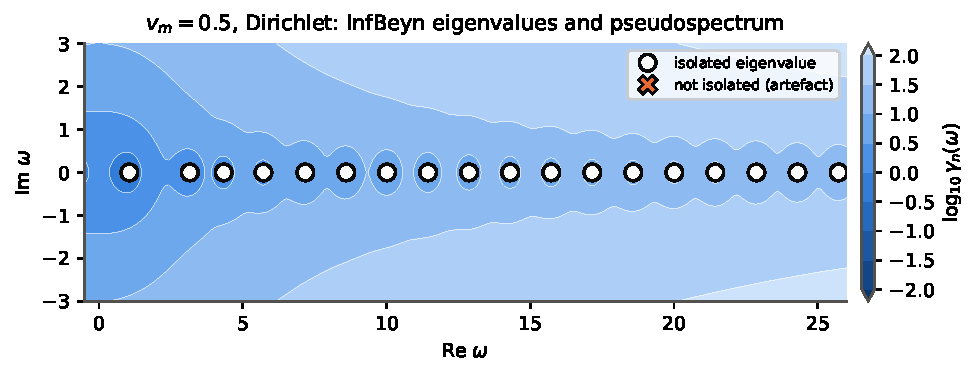
\includegraphics[width=\textwidth]{subsonic_fixed_fixed_spectrum}\\
  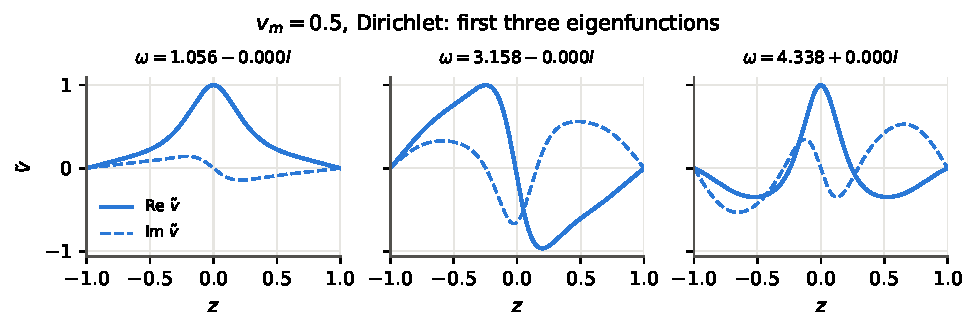
\includegraphics[width=\textwidth]{subsonic_fixed_fixed_eigenfunctions}
  \caption{Varying profile, $v_m=0.5$, Dirichlet.}
  \label{fig:ss}
\end{figure}
\begin{table}[H]\centering\footnotesize\begin{tabular}{rllll}
\toprule
$n$ & $\omega_n$ (InfBeyn) & $\gamma_{256}(\omega_n)$ & halo & polished\\
\midrule
1 & $1.05621525-0.00000000i$ & $1.4\times10^{-9}$ & $4.7\times10^{-1}$ & yes\\
2 & $3.15772808-0.00000000i$ & $1.3\times10^{-9}$ & $1.4\times10^{0}$ & yes\\
3 & $4.33790802+0.00000000i$ & $1.2\times10^{-9}$ & $2.0\times10^{0}$ & yes\\
4 & $5.71847609+0.00000000i$ & $1.3\times10^{-9}$ & $2.6\times10^{0}$ & yes\\
5 & $7.17529391-0.00000000i$ & $1.5\times10^{-9}$ & $3.3\times10^{0}$ & yes\\
6 & $8.59747157+0.00000000i$ & $1.4\times10^{-9}$ & $3.9\times10^{0}$ & yes\\
7 & $10.01903504-0.00000000i$ & $1.5\times10^{-9}$ & $4.6\times10^{0}$ & yes\\
8 & $11.44531362+0.00000000i$ & $1.5\times10^{-9}$ & $5.3\times10^{0}$ & yes\\
9 & $12.87226584-0.00000000i$ & $1.5\times10^{-9}$ & $5.9\times10^{0}$ & yes\\
10 & $14.29929220+0.00000000i$ & $1.4\times10^{-9}$ & $6.6\times10^{0}$ & yes\\
\bottomrule
\end{tabular}

  \caption{$v_m=0.5$, Dirichlet: first ten eigenvalues.}\label{tab:ss}\end{table}

\begin{figure}[H]
  \centering
  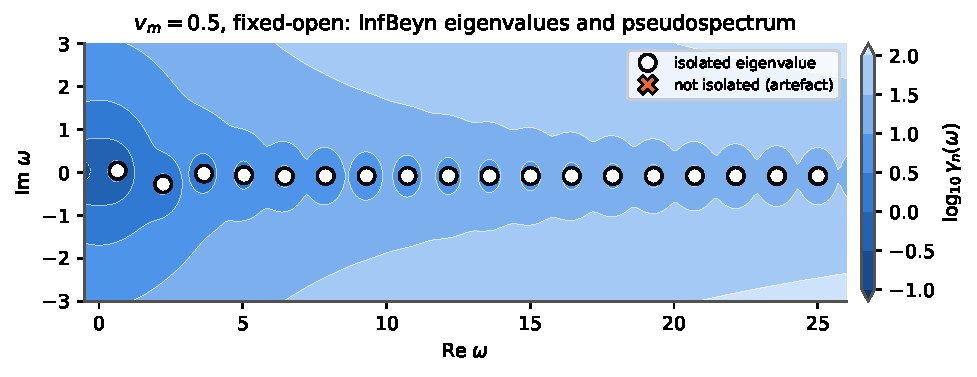
\includegraphics[width=\textwidth]{subsonic_fixed_open_spectrum}\\
  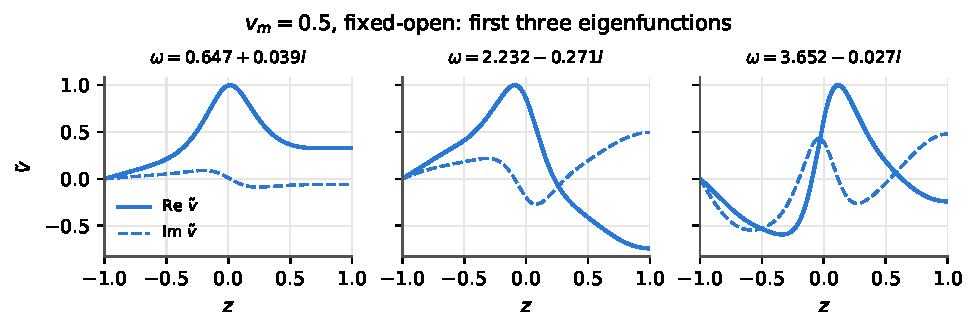
\includegraphics[width=\textwidth]{subsonic_fixed_open_eigenfunctions}
  \caption{Varying profile, $v_m=0.5$, fixed-open. Only the ground mode has $\Imag\omega>0$.}
  \label{fig:so}
\end{figure}
\begin{table}[H]\centering\footnotesize\begin{tabular}{rllll}
\toprule
$n$ & $\omega_n$ (InfBeyn) & $\gamma_{256}(\omega_n)$ & halo & polished\\
\midrule
1 & $0.64661598+0.03884264i$ & $1.4\times10^{-9}$ & $2.5\times10^{-1}$ & yes\\
2 & $2.23164113-0.27090622i$ & $2.2\times10^{-9}$ & $9.3\times10^{-1}$ & yes\\
3 & $3.65213616-0.02712519i$ & $1.6\times10^{-9}$ & $1.6\times10^{0}$ & yes\\
4 & $5.04410886-0.06304891i$ & $1.4\times10^{-9}$ & $2.3\times10^{0}$ & yes\\
5 & $6.46204378-0.09108792i$ & $1.5\times10^{-9}$ & $3.0\times10^{0}$ & yes\\
6 & $7.88229735-0.08332761i$ & $1.4\times10^{-9}$ & $3.7\times10^{0}$ & yes\\
7 & $9.30667567-0.08135647i$ & $1.6\times10^{-9}$ & $4.4\times10^{0}$ & yes\\
8 & $10.73237805-0.08227976i$ & $1.6\times10^{-9}$ & $5.0\times10^{0}$ & yes\\
9 & $12.15874297-0.08246613i$ & $1.5\times10^{-9}$ & $5.7\times10^{0}$ & yes\\
10 & $13.58561766-0.08240018i$ & $1.5\times10^{-9}$ & $6.4\times10^{0}$ & yes\\
\bottomrule
\end{tabular}

  \caption{$v_m=0.5$, fixed-open: first ten eigenvalues.}\label{tab:so}\end{table}

\begin{figure}[H]
  \centering
  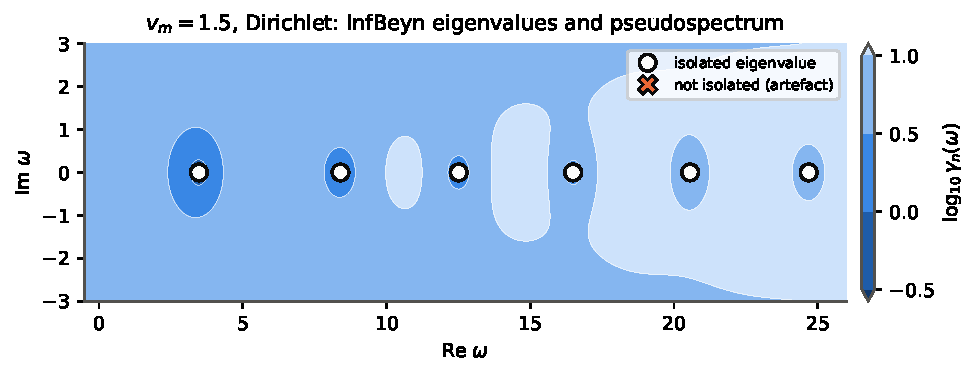
\includegraphics[width=\textwidth]{supersonic_fixed_fixed_spectrum}\\
  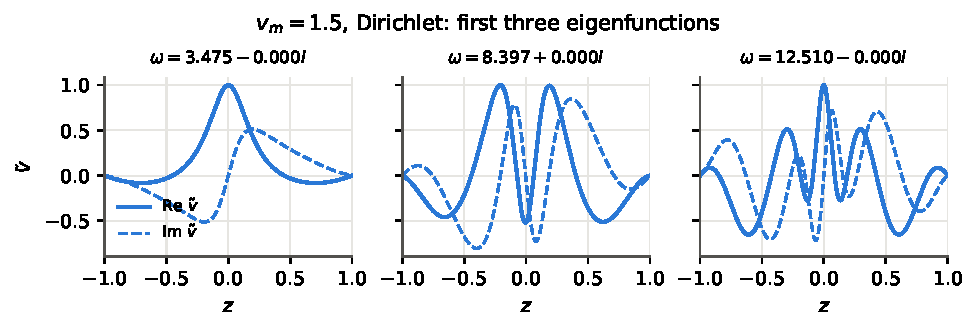
\includegraphics[width=\textwidth]{supersonic_fixed_fixed_eigenfunctions}
  \caption{Varying profile, $v_m=1.5$, Dirichlet.}
  \label{fig:Ss}
\end{figure}
\begin{table}[H]\centering\footnotesize\begin{tabular}{rllll}
\toprule
$n$ & $\omega_n$ (InfBeyn) & $\gamma_{256}(\omega_n)$ & halo & polished\\
\midrule
1 & $3.47455636-0.00000000i$ & $6.3\times10^{-9}$ & $8.2\times10^{-1}$ & yes\\
2 & $8.39673137+0.00000000i$ & $5.2\times10^{-9}$ & $1.4\times10^{0}$ & yes\\
3 & $12.51019598-0.00000000i$ & $6.4\times10^{-9}$ & $2.1\times10^{0}$ & yes\\
4 & $16.48904036+0.00000000i$ & $6.1\times10^{-9}$ & $2.8\times10^{0}$ & yes\\
5 & $20.55778685+0.00000000i$ & $6.5\times10^{-9}$ & $3.6\times10^{0}$ & yes\\
6 & $24.68263122+0.00000000i$ & $6.8\times10^{-9}$ & $4.3\times10^{0}$ & yes\\
\bottomrule
\end{tabular}

  \caption{$v_m=1.5$, Dirichlet: all six eigenvalues in the window.}\label{tab:Ss}\end{table}

\begin{figure}[H]
  \centering
  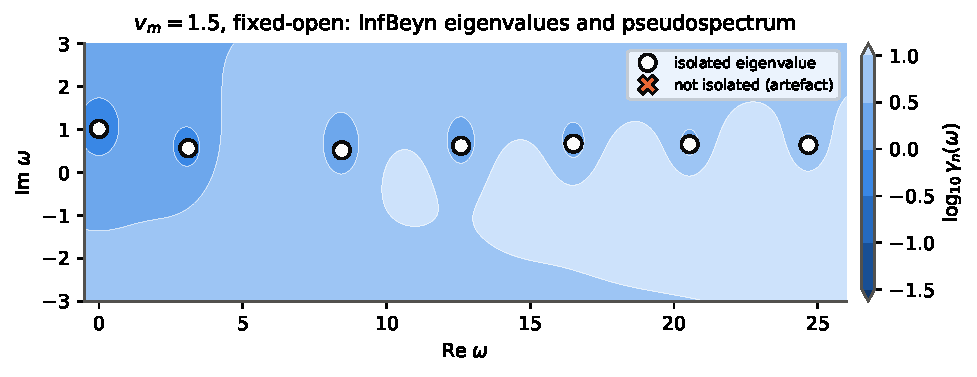
\includegraphics[width=\textwidth]{supersonic_fixed_open_spectrum}\\
  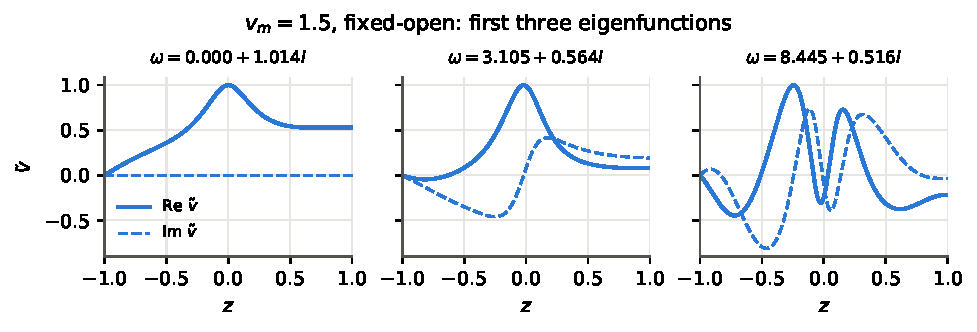
\includegraphics[width=\textwidth]{supersonic_fixed_open_eigenfunctions}
  \caption{Varying profile, $v_m=1.5$, fixed-open. Every mode is unstable.}
  \label{fig:So}
\end{figure}
\begin{table}[H]\centering\footnotesize\begin{tabular}{rllll}
\toprule
$n$ & $\omega_n$ (InfBeyn) & $\gamma_{256}(\omega_n)$ & halo & polished\\
\midrule
1 & $0.00000001+1.01356972i$ & $3.1\times10^{-8}$ & $3.8\times10^{-1}$ & no\\
2 & $3.10504212+0.56428533i$ & $4.6\times10^{-9}$ & $5.2\times10^{-1}$ & yes\\
3 & $8.44537466+0.51585847i$ & $3.5\times10^{-9}$ & $1.2\times10^{0}$ & yes\\
4 & $12.59137405+0.61963297i$ & $4.6\times10^{-9}$ & $1.5\times10^{0}$ & yes\\
5 & $16.50345376+0.67161842i$ & $5.4\times10^{-9}$ & $1.9\times10^{0}$ & yes\\
6 & $20.54359191+0.65642344i$ & $5.3\times10^{-9}$ & $2.4\times10^{0}$ & yes\\
7 & $24.67418498+0.64081281i$ & $5.1\times10^{-9}$ & $2.9\times10^{0}$ & yes\\
\bottomrule
\end{tabular}

  \caption{$v_m=1.5$, fixed-open: all seven eigenvalues in the window. See the text for the unpolished
  first mode.}\label{tab:So}\end{table}

\section{Comparison with the discretize-then-eig methods}

Figures~\ref{fig:cmp1}--\ref{fig:cmp4} overlay, for each case, every eigenvalue of the finite-difference
($N=101$, $201$), collocation and Galerkin discretizations that falls in the scanned window on the \infbeyn{}
eigenvalues, with a zoom on the imaginary parts of the first modes. Figures~\ref{fig:err1}--\ref{fig:err2}
show the distance from each \infbeyn{} eigenvalue to the nearest old eigenvalue, mode by mode, and for the
constant-velocity cases the distance from \infbeyn{} to the exact value. Tables~\ref{tab:cmp1}--\ref{tab:cmp4}
list the same distances and the number of spurious eigenvalues; Table~\ref{tab:spurious} collects the spurious
counts.

\begin{table}[H]
  \centering\small
  \begin{tabular}{llrrrrr}
\toprule
case & BC & InfBeyn & FD $N{=}101$ & FD $N{=}201$ & collocation & Galerkin\\
\midrule
constant $v_0=0.5$ & Dirichlet & 0 & 7 & 0 & 0 & 4\\
constant $v_0=0.5$ & fixed-open & 0 & 8 & 0 & 0 & 5\\
constant $v_0=1.5$ & Dirichlet & 0 & 7 & 7 & 0 & 2\\
constant $v_0=1.5$ & fixed-open & 0 & 8 & 7 & 0 & 1\\
$v_m=0.5$ & Dirichlet & 0 & 2 & 0 & 0 & 6\\
$v_m=0.5$ & fixed-open & 0 & 1 & 0 & 0 & 5\\
$v_m=1.5$ & Dirichlet & 0 & 4 & 3 & 0 & 3\\
$v_m=1.5$ & fixed-open & 0 & 4 & 3 & 0 & 3\\
\bottomrule
\end{tabular}

  \caption{Number of eigenvalues in the window $\Real\omega\in[-0.5,26]$, $\Imag\omega\in[-3,3]$ farther
  than $0.1$ from every \infbeyn{} eigenvalue (spurious), per method.}
  \label{tab:spurious}
\end{table}

\paragraph{Accuracy.} For the constant-velocity problems the exact solution settles the comparison:
\infbeyn{} and collocation both reach $10^{-13}$ to $10^{-12}$ on every mode in the window. Galerkin with 30
basis functions is as accurate for the first three modes and then loses one to two digits per mode
(thesis Fig.~4.9, 4.13, 4.15), down to $10^{-1}$ by mode 8 for $v_0=1.5$. Finite differences are second
order and their error grows like the square of the wavenumber: $10^{-3}$ on the first mode and $10^{-1}$ to
$10^{0}$ by mode 7 at $N=101$, four times smaller at $N=201$, which is consistent with the dispersion
analysis of thesis Sec.~4.4.1. For the varying profiles there is no exact solution, and \infbeyn{} is the most
accurate of the four, so the distances in Tables~\ref{tab:cmp3}, \ref{tab:cmp4} are the errors of the old
methods. Collocation at $N=101$ agrees with \infbeyn{} to $10^{-12}$--$10^{-10}$ with Dirichlet boundaries for both
profiles, but only to $10^{-3}$ with fixed-open boundaries ($1.2\times10^{-3}$ on the first subsonic mode,
$3.5\times10^{-3}$ on the first supersonic mode, $10^{-4}$ beyond). The loss is not a property of the collocation method but of the thesis-era script
(\texttt{archive/run\_experiments.py}): for the fixed-open case it rewrites one row of the Chebyshev
differentiation matrices in place to impose $\tilde v'(1)=0$, and then differentiates the equilibrium
profile with the same, already modified, matrices, so $v_0'$ and $v_0''$ are wrong at the grid point next to
$z=1$. Constant profiles (zero derivatives) and Dirichlet runs (no row rewriting) are unaffected, which is why
those agree to $10^{-12}$. Repeating the computation with copies of the matrices reproduces the stored
eigenvalues to $10^{-9}$ when the aliasing is kept and brings the collocation eigenvalues to within
$5\times10^{-8}$ ($v_m=1.5$) and $10^{-9}$ ($v_m=0.5$) of the \infbeyn{} values when it is removed.
The thesis statement that collocation and Galerkin
``agree well on the first three modes and start to deviate afterwards'' for $v_m=1.5$ (thesis Figs.~4.18,
4.19) is explained by Tables~\ref{tab:cmp4}: the collocation eigenvalues stay within $10^{-10}$ (Dirichlet)
or $10^{-3}$ (fixed-open) of the certified ones for all modes, while the Galerkin ones drift to $10^{-2}$
at mode 3 and to $10^{0}$ at mode 5. The Galerkin values, not the collocation ones, were the inaccurate ones.

\paragraph{Spurious eigenvalues.} Every discretization produces eigenvalues that are not eigenvalues of
the operator. Most of them have $|\Imag\omega|$ of order $10$ to $10^{3}$ and fall outside the window, but
Table~\ref{tab:spurious} shows that several remain inside it: up to 8 for finite differences at $N=101$ and
up to 6 for Galerkin, in every one of the eight cases. In the thesis they were removed by comparing two
resolutions (Sec.~4.4.2). \infbeyn{} produces none, because every eigenvalue it returns is a pole of the
resolvent inside a contour, confirmed by the rank gap, the nested quadrature rule, Newton polishing and
$\gamma_n$. Collocation at $N=101$ shows no spurious eigenvalue in the window for any case, but its
eigenvalues off the window (e.g.\ $\pm2245i$ for constant $v_0=1.5$) show that this is a property of the
window rather than of the method.

\paragraph{Completeness.} The scan also answers a question the old approach cannot: that there are no
further eigenvalues in the window. The pseudospectral plots are uniformly light away from the eigenvalues
(no hidden region of small $\gamma_n$), and the accepted tiles cover the entire window.

\begin{figure}[H]\centering
  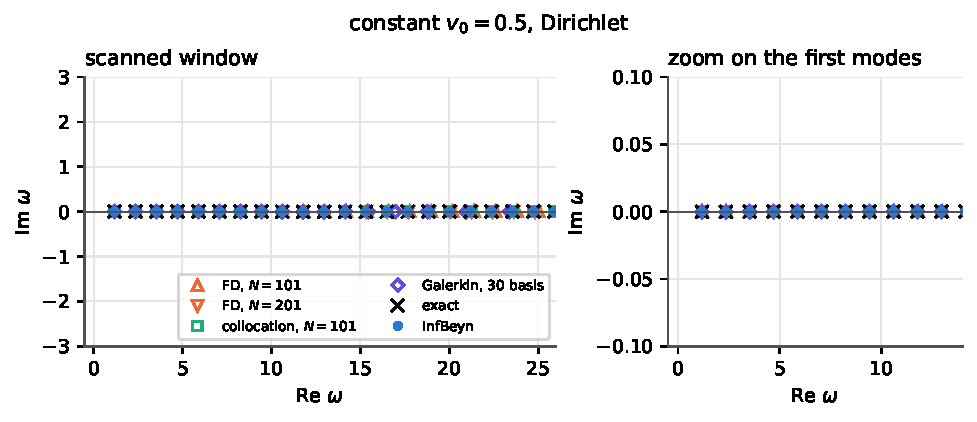
\includegraphics[width=\textwidth]{constant_subsonic_fixed_fixed_comparison}\\
  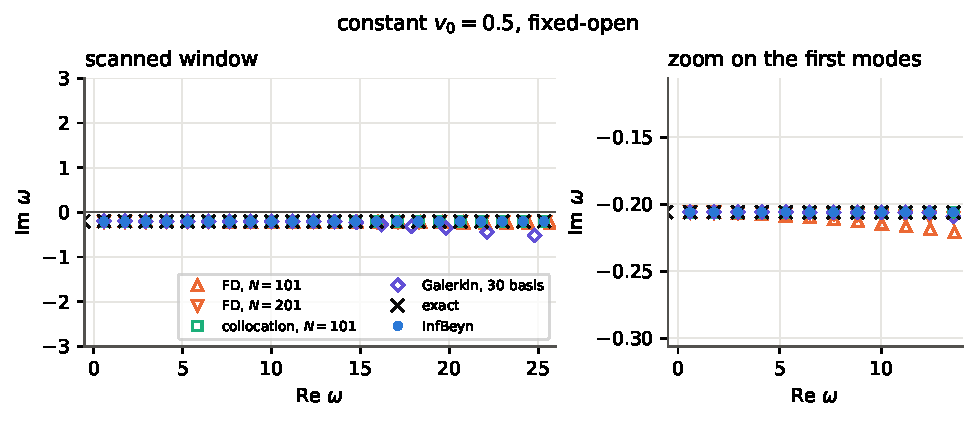
\includegraphics[width=\textwidth]{constant_subsonic_fixed_open_comparison}
  \caption{Constant $v_0=0.5$: all eigenvalues of the old discretizations in the window, with
  \infbeyn{} and exact values.}\label{fig:cmp1}\end{figure}
\begin{figure}[H]\centering
  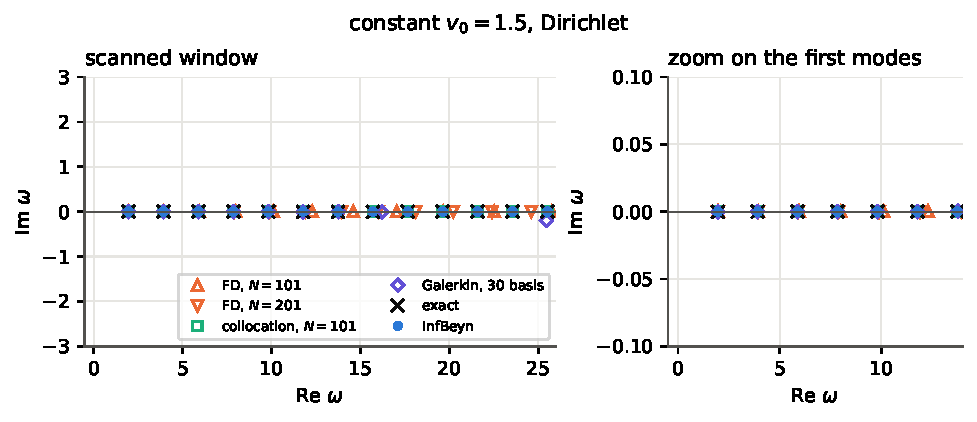
\includegraphics[width=\textwidth]{constant_supersonic_fixed_fixed_comparison}\\
  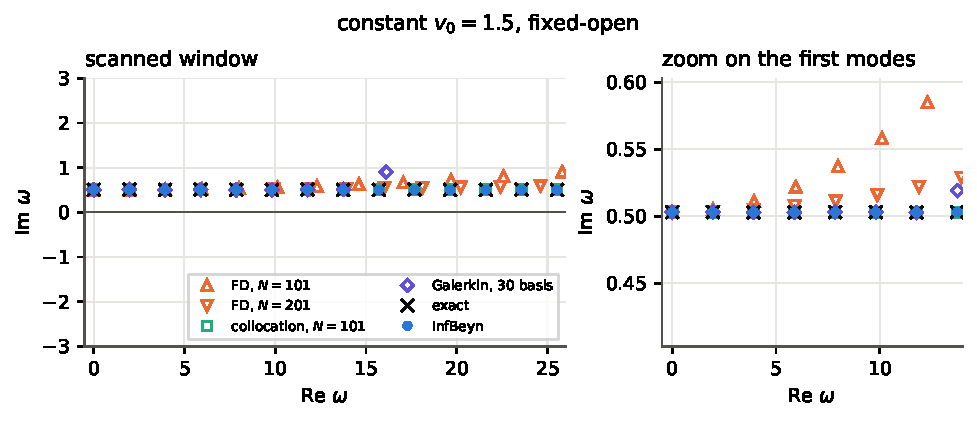
\includegraphics[width=\textwidth]{constant_supersonic_fixed_open_comparison}
  \caption{Constant $v_0=1.5$.}\label{fig:cmp2}\end{figure}
\begin{figure}[H]\centering
  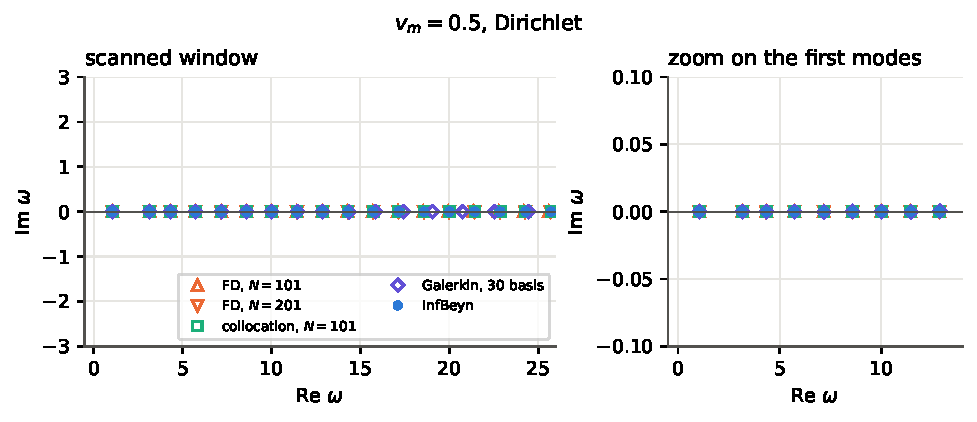
\includegraphics[width=\textwidth]{subsonic_fixed_fixed_comparison}\\
  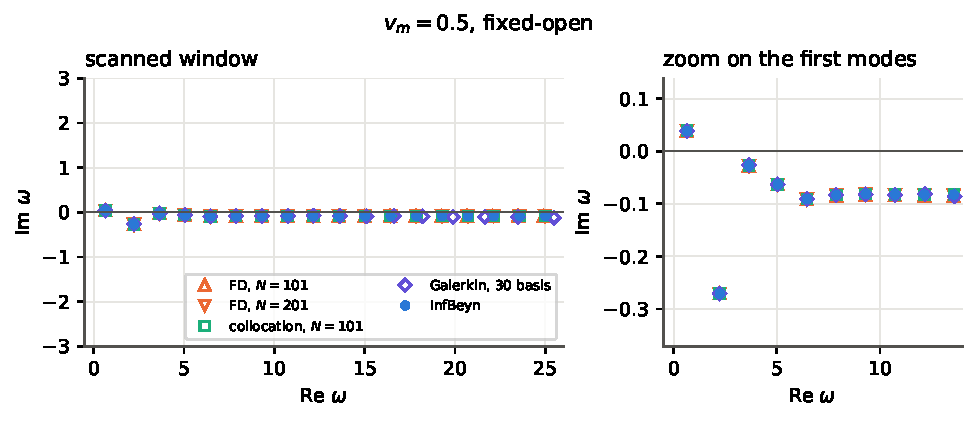
\includegraphics[width=\textwidth]{subsonic_fixed_open_comparison}
  \caption{Varying profile, $v_m=0.5$.}\label{fig:cmp3}\end{figure}
\begin{figure}[H]\centering
  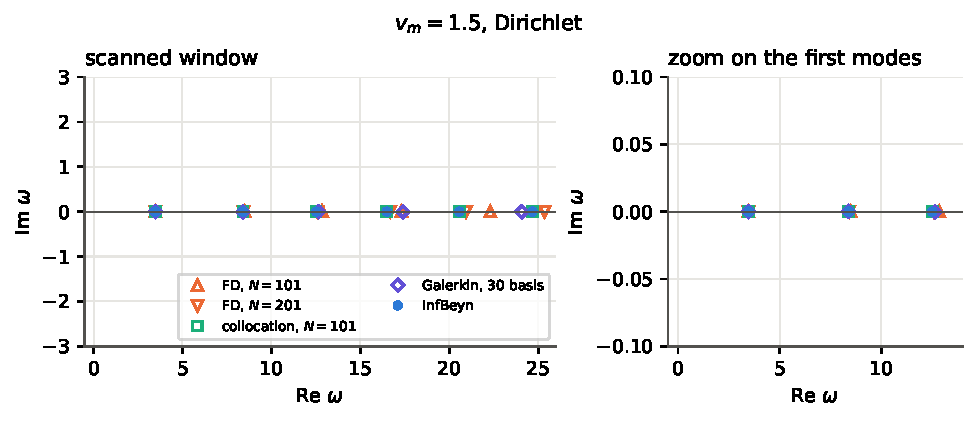
\includegraphics[width=\textwidth]{supersonic_fixed_fixed_comparison}\\
  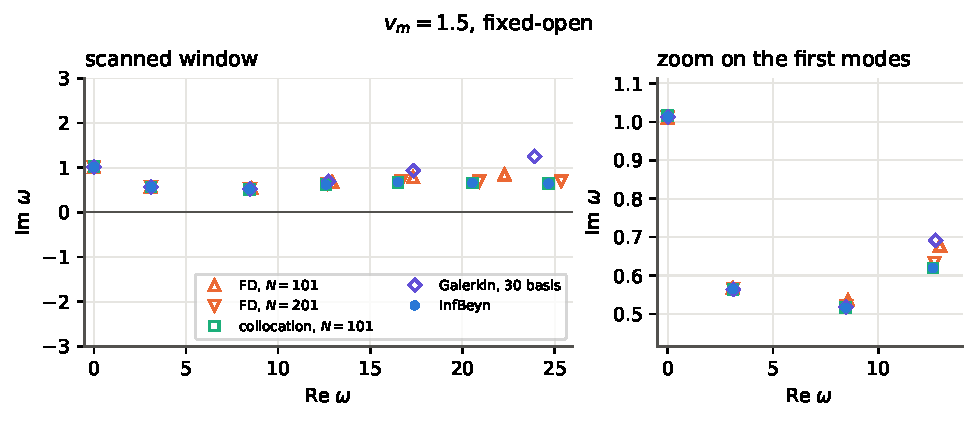
\includegraphics[width=\textwidth]{supersonic_fixed_open_comparison}
  \caption{Varying profile, $v_m=1.5$.}\label{fig:cmp4}\end{figure}

\begin{figure}[H]\centering
  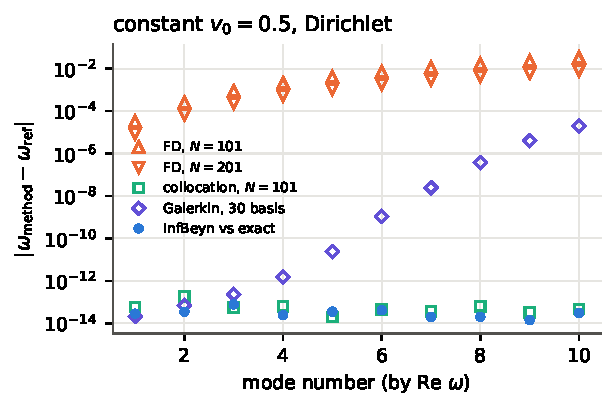
\includegraphics[width=0.49\textwidth]{constant_subsonic_fixed_fixed_errors}
  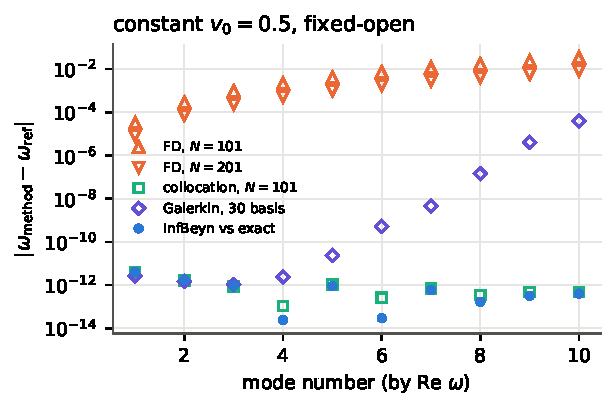
\includegraphics[width=0.49\textwidth]{constant_subsonic_fixed_open_errors}\\
  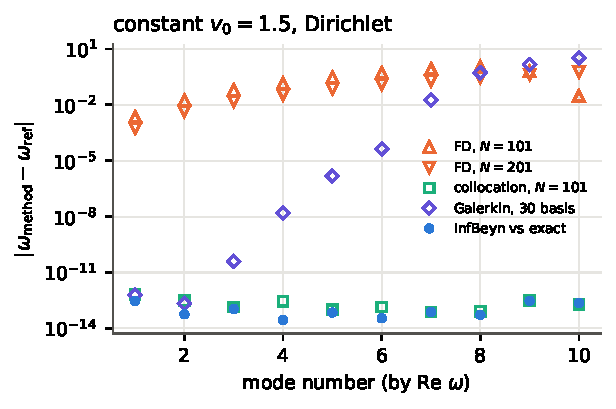
\includegraphics[width=0.49\textwidth]{constant_supersonic_fixed_fixed_errors}
  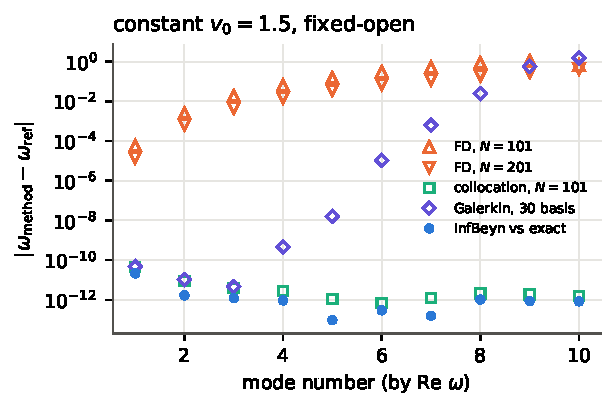
\includegraphics[width=0.49\textwidth]{constant_supersonic_fixed_open_errors}
  \caption{Constant velocity: distance from each \infbeyn{} eigenvalue to the nearest eigenvalue of each old
  method (open markers) and to the exact eigenvalue (filled circles), by mode number.}\label{fig:err1}\end{figure}
\begin{figure}[H]\centering
  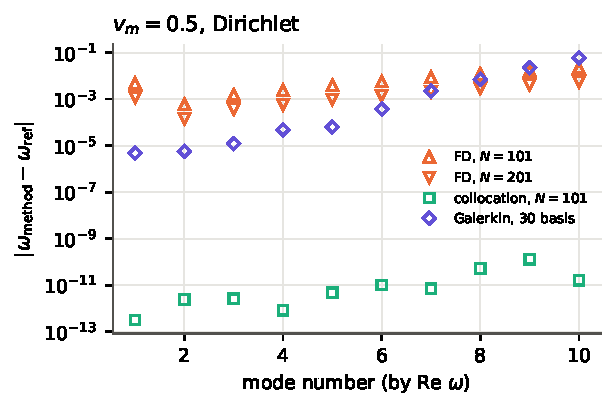
\includegraphics[width=0.49\textwidth]{subsonic_fixed_fixed_errors}
  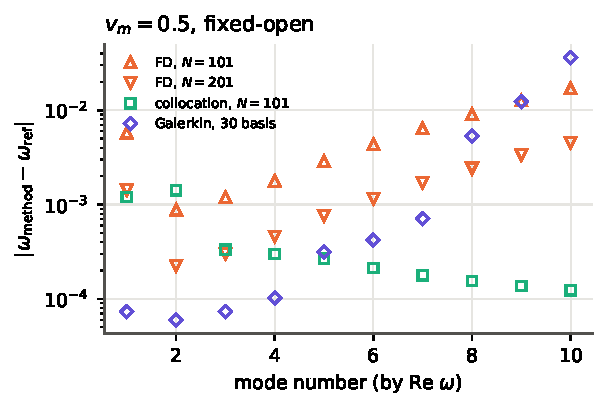
\includegraphics[width=0.49\textwidth]{subsonic_fixed_open_errors}\\
  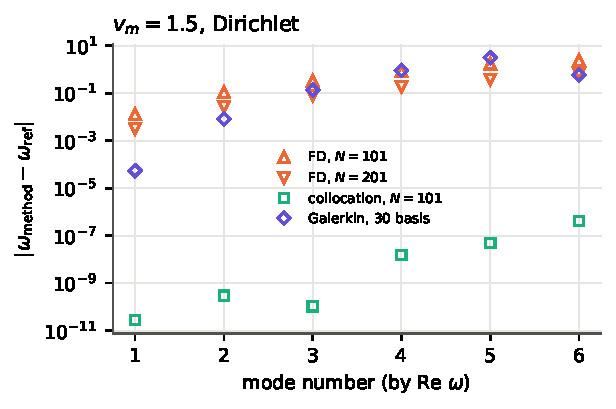
\includegraphics[width=0.49\textwidth]{supersonic_fixed_fixed_errors}
  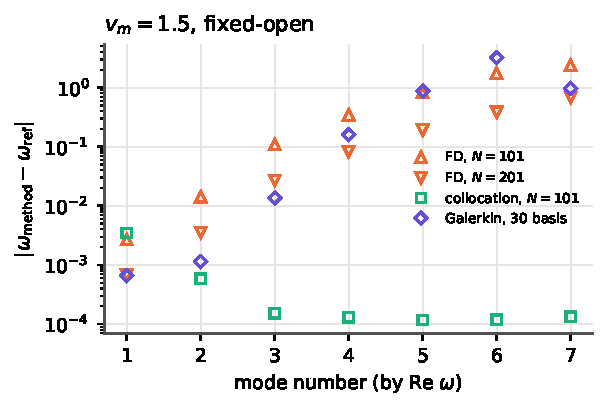
\includegraphics[width=0.49\textwidth]{supersonic_fixed_open_errors}
  \caption{Varying profiles: distance from each \infbeyn{} eigenvalue to the nearest eigenvalue of each old
  method.}\label{fig:err2}\end{figure}

\begin{table}[H]\centering\footnotesize
  \begin{tabular}{rllll}
\toprule
$n$ & FD, $N=101$ & FD, $N=201$ & collocation, $N=101$ & Galerkin, 30 basis\\
\midrule
1 & $3.3\times10^{-5}$ & $8.3\times10^{-6}$ & $5.9\times10^{-14}$ & $2.1\times10^{-14}$\\
2 & $2.7\times10^{-4}$ & $6.7\times10^{-5}$ & $1.9\times10^{-13}$ & $7.1\times10^{-14}$\\
3 & $9.0\times10^{-4}$ & $2.2\times10^{-4}$ & $5.6\times10^{-14}$ & $2.3\times10^{-13}$\\
4 & $2.1\times10^{-3}$ & $5.3\times10^{-4}$ & $6.3\times10^{-14}$ & $1.5\times10^{-12}$\\
5 & $4.1\times10^{-3}$ & $1.0\times10^{-3}$ & $2.0\times10^{-14}$ & $2.4\times10^{-11}$\\
6 & $7.2\times10^{-3}$ & $1.8\times10^{-3}$ & $4.6\times10^{-14}$ & $1.1\times10^{-9}$\\
7 & $1.1\times10^{-2}$ & $2.9\times10^{-3}$ & $3.7\times10^{-14}$ & $2.5\times10^{-8}$\\
8 & $1.7\times10^{-2}$ & $4.3\times10^{-3}$ & $6.4\times10^{-14}$ & $3.8\times10^{-7}$\\
\midrule
in window & 21 & 21 & 22 & 17\\
spurious & 7 & 0 & 0 & 4\\
\bottomrule
\end{tabular}
\quad\begin{tabular}{rllll}
\toprule
$n$ & FD, $N=101$ & FD, $N=201$ & collocation, $N=101$ & Galerkin, 30 basis\\
\midrule
1 & $3.3\times10^{-5}$ & $8.2\times10^{-6}$ & $3.7\times10^{-12}$ & $2.7\times10^{-12}$\\
2 & $3.0\times10^{-4}$ & $7.3\times10^{-5}$ & $1.7\times10^{-12}$ & $1.5\times10^{-12}$\\
3 & $9.4\times10^{-4}$ & $2.3\times10^{-4}$ & $8.6\times10^{-13}$ & $1.0\times10^{-12}$\\
4 & $2.2\times10^{-3}$ & $5.2\times10^{-4}$ & $1.1\times10^{-13}$ & $2.4\times10^{-12}$\\
5 & $4.2\times10^{-3}$ & $1.0\times10^{-3}$ & $1.1\times10^{-12}$ & $2.4\times10^{-11}$\\
6 & $7.2\times10^{-3}$ & $1.7\times10^{-3}$ & $2.6\times10^{-13}$ & $5.2\times10^{-10}$\\
7 & $1.1\times10^{-2}$ & $2.7\times10^{-3}$ & $7.1\times10^{-13}$ & $4.5\times10^{-9}$\\
8 & $1.7\times10^{-2}$ & $4.1\times10^{-3}$ & $3.5\times10^{-13}$ & $1.4\times10^{-7}$\\
\midrule
in window & 22 & 22 & 22 & 18\\
spurious & 8 & 0 & 0 & 5\\
\bottomrule
\end{tabular}

  \caption{Constant $v_0=0.5$, Dirichlet (left) and fixed-open (right): $|\omega_n^{\rm method}-\omega_n^{\rm InfBeyn}|$
  for the first eight modes, number of old eigenvalues in the window and number of spurious ones.}\label{tab:cmp1}\end{table}
\begin{table}[H]\centering\footnotesize
  \begin{tabular}{rllll}
\toprule
$n$ & FD, $N=101$ & FD, $N=201$ & collocation, $N=101$ & Galerkin, 30 basis\\
\midrule
1 & $2.2\times10^{-3}$ & $5.6\times10^{-4}$ & $6.5\times10^{-13}$ & $6.2\times10^{-13}$\\
2 & $1.8\times10^{-2}$ & $4.5\times10^{-3}$ & $3.1\times10^{-13}$ & $2.2\times10^{-13}$\\
3 & $6.2\times10^{-2}$ & $1.5\times10^{-2}$ & $1.4\times10^{-13}$ & $4.0\times10^{-11}$\\
4 & $1.5\times10^{-1}$ & $3.6\times10^{-2}$ & $2.9\times10^{-13}$ & $1.5\times10^{-8}$\\
5 & $3.0\times10^{-1}$ & $7.1\times10^{-2}$ & $1.0\times10^{-13}$ & $1.5\times10^{-6}$\\
6 & $5.2\times10^{-1}$ & $1.2\times10^{-1}$ & $1.4\times10^{-13}$ & $4.3\times10^{-5}$\\
7 & $8.6\times10^{-1}$ & $2.0\times10^{-1}$ & $7.6\times10^{-14}$ & $1.9\times10^{-2}$\\
8 & $1.1\times10^{0}$ & $3.0\times10^{-1}$ & $8.0\times10^{-14}$ & $5.2\times10^{-1}$\\
\midrule
in window & 11 & 12 & 13 & 9\\
spurious & 7 & 7 & 0 & 2\\
\bottomrule
\end{tabular}
\quad\begin{tabular}{rllll}
\toprule
$n$ & FD, $N=101$ & FD, $N=201$ & collocation, $N=101$ & Galerkin, 30 basis\\
\midrule
1 & $5.9\times10^{-5}$ & $1.5\times10^{-5}$ & $4.6\times10^{-11}$ & $4.8\times10^{-11}$\\
2 & $2.6\times10^{-3}$ & $6.5\times10^{-4}$ & $8.9\times10^{-12}$ & $1.0\times10^{-11}$\\
3 & $1.9\times10^{-2}$ & $4.7\times10^{-3}$ & $3.9\times10^{-12}$ & $4.6\times10^{-12}$\\
4 & $6.4\times10^{-2}$ & $1.6\times10^{-2}$ & $2.8\times10^{-12}$ & $4.7\times10^{-10}$\\
5 & $1.5\times10^{-1}$ & $3.7\times10^{-2}$ & $1.1\times10^{-12}$ & $1.6\times10^{-8}$\\
6 & $3.0\times10^{-1}$ & $7.2\times10^{-2}$ & $6.9\times10^{-13}$ & $1.1\times10^{-5}$\\
7 & $5.3\times10^{-1}$ & $1.2\times10^{-1}$ & $1.3\times10^{-12}$ & $6.2\times10^{-4}$\\
8 & $8.8\times10^{-1}$ & $2.0\times10^{-1}$ & $2.1\times10^{-12}$ & $2.5\times10^{-2}$\\
\midrule
in window & 12 & 13 & 14 & 9\\
spurious & 8 & 7 & 0 & 1\\
\bottomrule
\end{tabular}

  \caption{Constant $v_0=1.5$, Dirichlet (left) and fixed-open (right).}\label{tab:cmp2}\end{table}
\begin{table}[H]\centering\footnotesize
  \begin{tabular}{rllll}
\toprule
$n$ & FD, $N=101$ & FD, $N=201$ & collocation, $N=101$ & Galerkin, 30 basis\\
\midrule
1 & $4.8\times10^{-3}$ & $1.2\times10^{-3}$ & $3.2\times10^{-13}$ & $4.7\times10^{-6}$\\
2 & $5.8\times10^{-4}$ & $1.5\times10^{-4}$ & $2.4\times10^{-12}$ & $5.8\times10^{-6}$\\
3 & $1.5\times10^{-3}$ & $3.8\times10^{-4}$ & $2.6\times10^{-12}$ & $1.2\times10^{-5}$\\
4 & $2.4\times10^{-3}$ & $5.9\times10^{-4}$ & $8.4\times10^{-13}$ & $4.9\times10^{-5}$\\
5 & $3.9\times10^{-3}$ & $9.7\times10^{-4}$ & $4.8\times10^{-12}$ & $6.4\times10^{-5}$\\
6 & $5.7\times10^{-3}$ & $1.4\times10^{-3}$ & $1.0\times10^{-11}$ & $3.7\times10^{-4}$\\
7 & $8.5\times10^{-3}$ & $2.1\times10^{-3}$ & $7.2\times10^{-12}$ & $2.2\times10^{-3}$\\
8 & $1.2\times10^{-2}$ & $3.0\times10^{-3}$ & $5.2\times10^{-11}$ & $7.1\times10^{-3}$\\
\midrule
in window & 18 & 18 & 18 & 16\\
spurious & 2 & 0 & 0 & 6\\
\bottomrule
\end{tabular}
\quad\begin{tabular}{rllll}
\toprule
$n$ & FD, $N=101$ & FD, $N=201$ & collocation, $N=101$ & Galerkin, 30 basis\\
\midrule
1 & $5.8\times10^{-3}$ & $1.4\times10^{-3}$ & $1.2\times10^{-3}$ & $7.3\times10^{-5}$\\
2 & $8.8\times10^{-4}$ & $2.2\times10^{-4}$ & $1.4\times10^{-3}$ & $6.0\times10^{-5}$\\
3 & $1.2\times10^{-3}$ & $3.0\times10^{-4}$ & $3.3\times10^{-4}$ & $7.3\times10^{-5}$\\
4 & $1.8\times10^{-3}$ & $4.6\times10^{-4}$ & $3.0\times10^{-4}$ & $1.0\times10^{-4}$\\
5 & $2.9\times10^{-3}$ & $7.5\times10^{-4}$ & $2.7\times10^{-4}$ & $3.1\times10^{-4}$\\
6 & $4.3\times10^{-3}$ & $1.1\times10^{-3}$ & $2.1\times10^{-4}$ & $4.2\times10^{-4}$\\
7 & $6.4\times10^{-3}$ & $1.7\times10^{-3}$ & $1.8\times10^{-4}$ & $7.1\times10^{-4}$\\
8 & $9.1\times10^{-3}$ & $2.4\times10^{-3}$ & $1.6\times10^{-4}$ & $5.3\times10^{-3}$\\
\midrule
in window & 18 & 18 & 18 & 17\\
spurious & 1 & 0 & 0 & 5\\
\bottomrule
\end{tabular}

  \caption{Varying $v_m=0.5$, Dirichlet (left) and fixed-open (right).}\label{tab:cmp3}\end{table}
\begin{table}[H]\centering\footnotesize
  \begin{tabular}{rllll}
\toprule
$n$ & FD, $N=101$ & FD, $N=201$ & collocation, $N=101$ & Galerkin, 30 basis\\
\midrule
1 & $1.3\times10^{-2}$ & $3.2\times10^{-3}$ & $2.8\times10^{-11}$ & $5.5\times10^{-5}$\\
2 & $1.1\times10^{-1}$ & $2.7\times10^{-2}$ & $3.0\times10^{-10}$ & $8.1\times10^{-3}$\\
3 & $3.4\times10^{-1}$ & $8.1\times10^{-2}$ & $1.1\times10^{-10}$ & $1.4\times10^{-1}$\\
4 & $8.3\times10^{-1}$ & $1.9\times10^{-1}$ & $1.5\times10^{-8}$ & $9.1\times10^{-1}$\\
5 & $1.7\times10^{0}$ & $3.8\times10^{-1}$ & $4.9\times10^{-8}$ & $3.2\times10^{0}$\\
6 & $2.4\times10^{0}$ & $6.8\times10^{-1}$ & $4.2\times10^{-7}$ & $6.0\times10^{-1}$\\
\midrule
in window & 5 & 6 & 6 & 5\\
spurious & 4 & 3 & 0 & 3\\
\bottomrule
\end{tabular}
\quad\begin{tabular}{rllll}
\toprule
$n$ & FD, $N=101$ & FD, $N=201$ & collocation, $N=101$ & Galerkin, 30 basis\\
\midrule
1 & $2.7\times10^{-3}$ & $6.7\times10^{-4}$ & $3.5\times10^{-3}$ & $6.6\times10^{-4}$\\
2 & $1.4\times10^{-2}$ & $3.5\times10^{-3}$ & $5.8\times10^{-4}$ & $1.1\times10^{-3}$\\
3 & $1.1\times10^{-1}$ & $2.7\times10^{-2}$ & $1.5\times10^{-4}$ & $1.4\times10^{-2}$\\
4 & $3.4\times10^{-1}$ & $8.2\times10^{-2}$ & $1.3\times10^{-4}$ & $1.6\times10^{-1}$\\
5 & $8.3\times10^{-1}$ & $1.9\times10^{-1}$ & $1.2\times10^{-4}$ & $8.7\times10^{-1}$\\
6 & $1.8\times10^{0}$ & $3.8\times10^{-1}$ & $1.2\times10^{-4}$ & $3.2\times10^{0}$\\
7 & $2.4\times10^{0}$ & $6.8\times10^{-1}$ & $1.3\times10^{-4}$ & $9.7\times10^{-1}$\\
\midrule
in window & 6 & 7 & 7 & 6\\
spurious & 4 & 3 & 0 & 3\\
\bottomrule
\end{tabular}

  \caption{Varying $v_m=1.5$, Dirichlet (left) and fixed-open (right).}\label{tab:cmp4}\end{table}

\section{Conclusions}

\begin{itemize}
  \item \infbeyn{} reproduces all stability verdicts of the thesis for the non-transonic flows, now with a
  certificate for each eigenvalue and a guarantee that no eigenvalue in the window was missed. No
  convergence test or spurious-mode filtering is needed.
  \item For constant velocity the eigenvalues agree with the exact ones to $10^{-13}$ (to $10^{-11}$ for the
  purely imaginary fixed-open supersonic mode). The thesis-era collocation is equally accurate there; finite
  differences and Galerkin are not.
  \item For the varying profiles the collocation results of the thesis are accurate to $10^{-10}$ with
  Dirichlet and, because of an aliasing slip in the old script, only to $10^{-3}$ with fixed-open boundaries
  (to $10^{-8}$ once the slip is removed); the disagreement between collocation and Galerkin above the third
  mode reported in the thesis is due to the Galerkin values.
  \item Thesis Eq.~(3.12) should read with phase $(2n+1)\pi/4$ for $v_0<1$; the figures of the thesis
  already use the correct values.
  \item Certified growth rates: $0.50295$ (constant $v_0=1.5$, fixed-open, all modes), $0.03884$ (varying
  $v_m=0.5$, fixed-open, ground mode only) and $1.01357$ (varying $v_m=1.5$, fixed-open, $\Real\omega=0$ mode).
\end{itemize}

\paragraph{Reproduction.} From the repository root:
\texttt{uv run python nontransonic\_flow/nozzle\_infbeyn.py} (about 2.5 minutes on 12 cores, writes
\texttt{nontransonic\_flow/data/infbeyn\_*.npz}), then
\texttt{uv run python nontransonic\_flow/make\_figures.py} and
\texttt{tectonic nontransonic\_flow/report.tex}.

\begin{thebibliography}{9}
\bibitem{feng2024} H.~Feng, \emph{Spectral stability of plasma flows in the magnetic nozzle}, M.Sc.\ thesis,
University of Saskatchewan, 2024.
\bibitem{colbrook2023} M.~J.~Colbrook and A.~Townsend, \emph{Avoiding discretization issues for nonlinear
eigenvalue problems}, arXiv:2305.01691, 2023.
\end{thebibliography}

\end{document}
